\chapter{Wizualizacja przy pomocy warstw ukrytych sieci VGG-19}
\label{chap:vgg}
\section{Model sieci VGG-19}
\label{vgg-model}

Do bardziej złożonych wizualizacji posłużę się siecią VGG, której architekturę zaprezentowano po raz pierwszy w 2015 roku w publikacji autorstwa Karen Simonyan i 
Andrew Zisserman\cite{vggpaper}. W publikacji zaprezentowano kilka wariantów tej sieci, ja z uwagi na większą ilość warstw użyję wariantu VGG-19.

\begin{figure}[ht]
\centerline{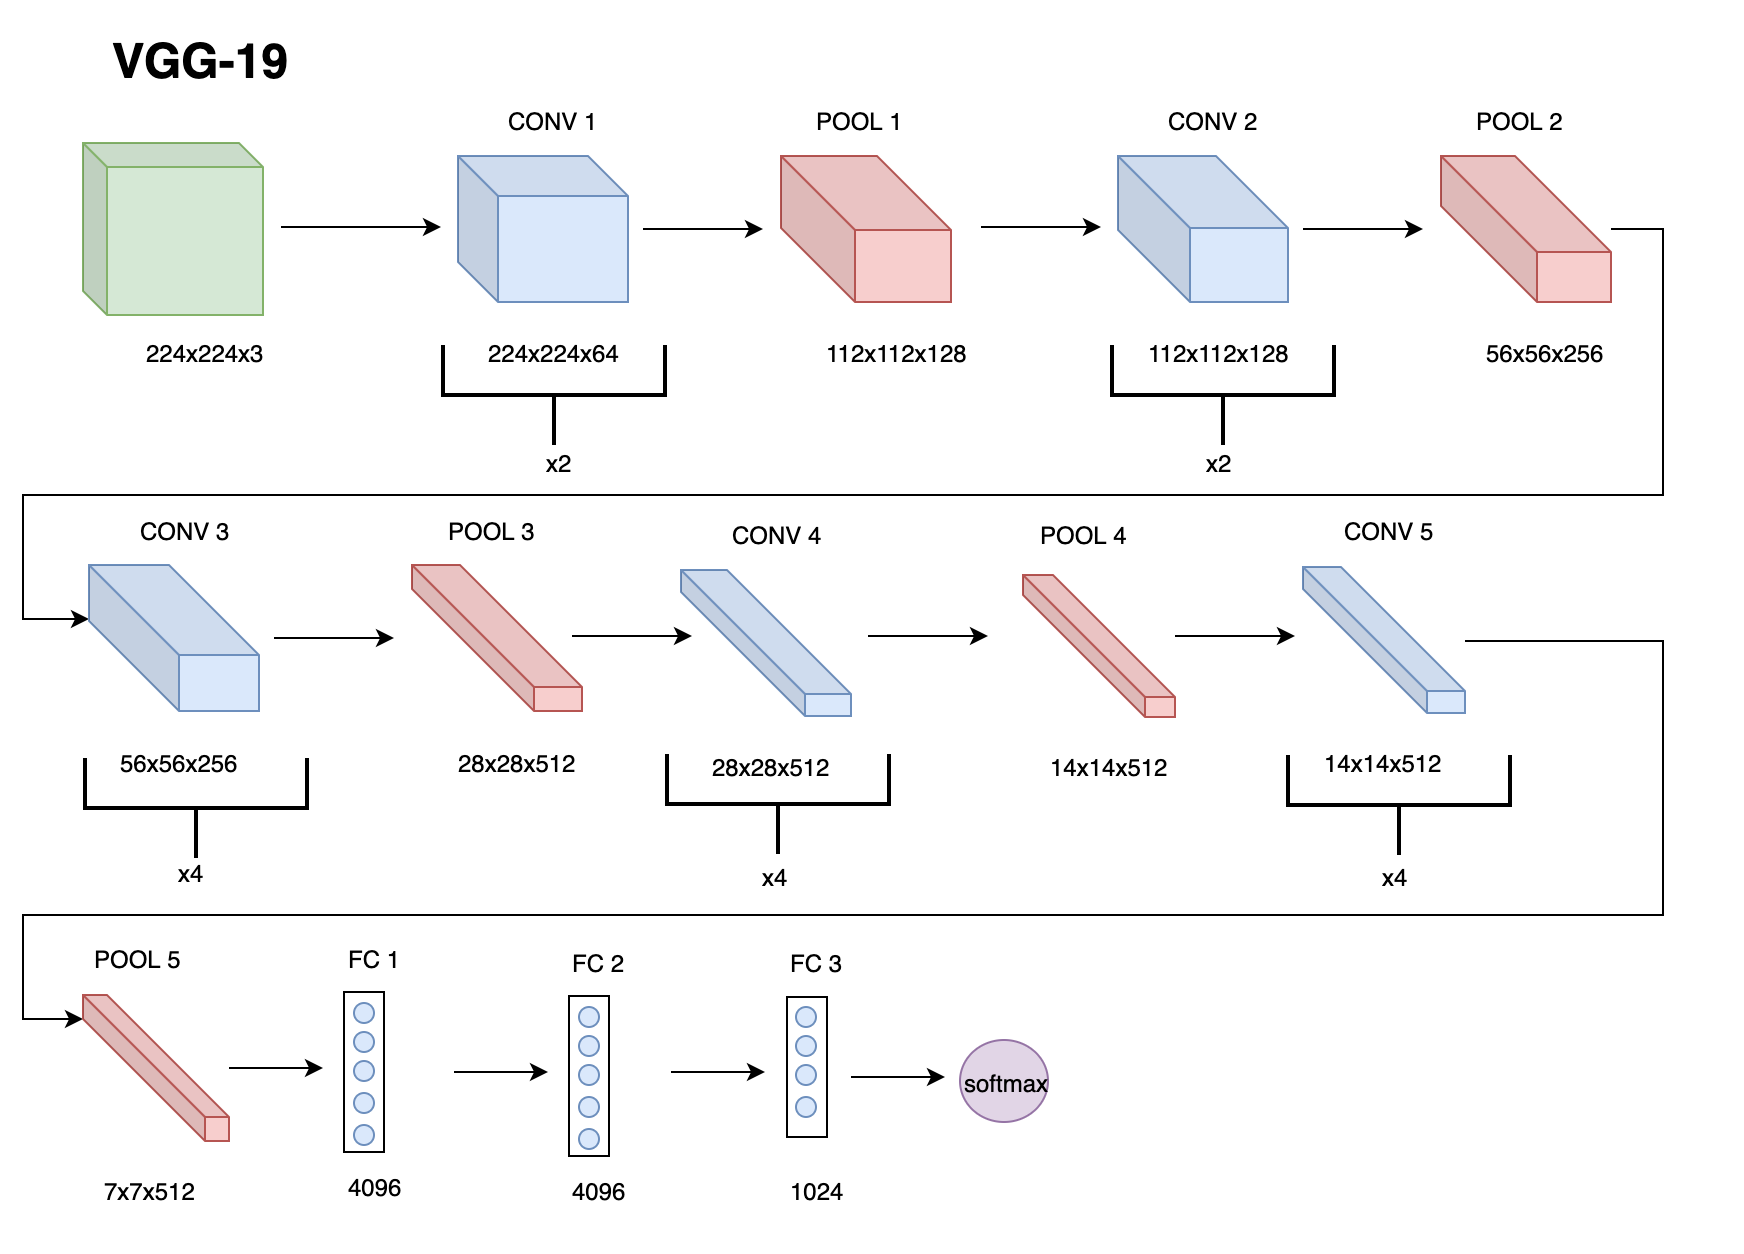
\includegraphics[scale=0.5]{resources/vgg19.png}}
\caption{Schemat modelu sieci VGG-19.}
\label{fig:vgg19-schemat}
\end{figure}

Dopełnienie w przypadku warstw konwolucyjnych wynosi \(p=1\) przy skoku \(s=1\) co sprawia, że warstwy konwolucyjne mogą być ze sobą łączone w łańcuchy niezmieniające wymiarów tensora. W przypadku warstw poolingowych \(p=1\) przy skoku \(s=2\) tym samym, dzielą one dwa pierwsze wymiary przez pół. Sumarycznie daje to 16 warstw możliwych do wykorzystania w wizualizacjach.

\subsection{Wizualizacja sieci VGG poprzez rekonstrukcję obrazu przy pomocy maksymalizacji aktywacji neuronu.}
\label{vgg-mean-activation}

Z racji swoich rozmiarów trening sieci VGG potrafi trwać dniami, nawet przy pomocy GPU. Użyję więc wcześniej wytrenowanej sieci dostępnej bezpośrednio w Kerasie.

\label{lst:vggkeras}
\begin{lstlisting}[language=Python, caption={Wczytywanie wag VGG-19 w Keras.}, captionpos=b]
from keras.applications import VGG19
model = VGG19(include_top=False, weights='imagenet')
\end{lstlisting}

Zastosowane opcje to przedewszystkim zestaw danych na których była trenowana sieć, w tym wypadku zbiór 
%ImagerNet\cite{ImageNet-dataset}.
